\chapter{Revisão da Literatura}
\citeonline{Moh06} desenvolveram um trabalho utilizando MD no qual o objetivo foi desenvolver modelos para classificação de doenças do arroz egípcio. Um dos algoritmos de aprendizagem utilizado foi a RNA. A RNA foi construída e treinada utilizando uma configuração de 52 entradas, 33 neurônios na camada oculta, 5 saídas, taxa de aprendizagem de 0.3, momento de 0.2 e 500 iterações. O modelo obtido para a previsão de doenças de arroz atingiu um índice de acerto de 96,4\% para o conjunto de dados de teste. Este resultado demonstra a grande eficiência da aplicação de RNAs.

O processo de mineração de dados é ilustrado na Figura~\ref{fig:mineracao}.
\begin{figure}
	\centering
	\caption{Etapas da mineração de dados}\label{fig:mineracao}
	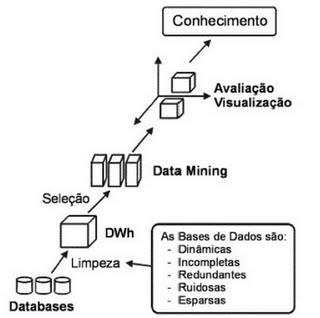
\includegraphics[scale=1.0]{mineracao}
	
\end{figure}


